%
%Не забыть:
%--------------------------------------
%Вставить колонтитулы, поменять название на титульнике



%--------------------------------------

\documentclass[a4paper, 12pt]{article} 

%--------------------------------------
%Russian-specific packages
%--------------------------------------
%\usepackage[warn]{mathtext}
\usepackage[T2A]{fontenc}
\usepackage[utf8]{inputenc}
\usepackage[english,russian]{babel}
\usepackage[intlimits]{amsmath}
\usepackage{esint}
%--------------------------------------
%Hyphenation rules
%--------------------------------------
\usepackage{hyphenat}
\hyphenation{ма-те-ма-ти-ка вос-ста-нав-ли-вать}
%--------------------------------------
%Packages
%--------------------------------------
\usepackage{amsmath}
\usepackage{amssymb}
\usepackage{amsfonts}
\usepackage{amsthm}
\usepackage{latexsym}
\usepackage{mathtools}
\usepackage{etoolbox}%Булевые операторы
\usepackage{extsizes}%Выставление произвольного шрифта в \documentclass
\usepackage{geometry}%Разметка листа
\usepackage{indentfirst}
\usepackage{wrapfig}%Создание обтекаемых текстом объектов
\usepackage{fancyhdr}%Создание колонтитулов
\usepackage{setspace}%Настройка интерлиньяжа
\usepackage{lastpage}%Вывод номера последней страницы в документе, \lastpage
\usepackage{soul}%Изменение параметров начертания
\usepackage{hyperref}%Две строчки с настройкой гиперссылок внутри получаеммого
\usepackage[usenames,dvipsnames,svgnames,table,rgb]{xcolor}% pdf-документа
\usepackage{multicol}%Позволяет писать текст в несколько колонок
\usepackage{cite}%Работа с библиографией
\usepackage{subfigure}% Человеческая вставка нескольких картинок
\usepackage{tikz}%Рисование рисунков
\usepackage{float}% Возможность ставить H в положениях картинки
% Для картинок Моти
\usepackage{misccorr}
\usepackage{lscape}
\usepackage{cmap}



\usepackage{graphicx,xcolor}
\graphicspath{{Pictures/}}
\DeclareGraphicsExtensions{.pdf,.png,.jpg}

%----------------------------------------
%Список окружений
%----------------------------------------
\newenvironment {theor}[2]
{\smallskip \par \textbf{#1.} \textit{#2}  \par $\blacktriangleleft$}
{\flushright{$\blacktriangleright$} \medskip \par} %лемма/теорема с доказательством
\newenvironment {proofn}
{\par $\blacktriangleleft$}
{$\blacktriangleright$ \par} %доказательство
%----------------------------------------
%Список команд
%----------------------------------------
\newcommand{\grad}
{\mathop{\mathrm{grad}}\nolimits\,} %градиент

\newcommand{\diver}
{\mathop{\mathrm{div}}\nolimits\,} %дивергенция

\newcommand{\rot}
{\ensuremath{\mathrm{rot}}\,}

\newcommand{\Def}[1]
{\underline{\textbf{#1}}} %определение

\newcommand{\RN}[1]
{\MakeUppercase{\romannumeral #1}} %римские цифры

\newcommand {\theornp}[2]
{\textbf{#1.} \textit{ #2} \par} %Написание леммы/теоремы без доказательства

\newcommand{\qrq}
{\ensuremath{\quad \Rightarrow \quad}} %Человеческий знак следствия

\newcommand{\qlrq}
{\ensuremath{\quad \Leftrightarrow \quad}} %Человеческий знак равносильности

\renewcommand{\phi}{\varphi} %Нормальный знак фи

\newcommand{\me}
{\ensuremath{\mathbb{E}}}

\newcommand{\md}
{\ensuremath{\mathbb{D}}}



%\renewcommand{\vec}{\overline}




%----------------------------------------
%Разметка листа
%----------------------------------------
\geometry{top = 3cm}
\geometry{bottom = 2cm}
\geometry{left = 1.5cm}
\geometry{right = 1.5cm}
%----------------------------------------
%Колонтитулы
%----------------------------------------
\pagestyle{fancy}%Создание колонтитулов
\fancyhead{}
%\fancyfoot{}
\fancyhead[R]{\textsc{Изучение центрированных оптических систем}}%Вставить колонтитул сюда
%----------------------------------------
%Интерлиньяж (расстояния между строчками)
%----------------------------------------
%\onehalfspacing -- интерлиньяж 1.5
%\doublespacing -- интерлиньяж 2
%----------------------------------------
%Настройка гиперссылок
%----------------------------------------
\hypersetup{				% Гиперссылки
	unicode=true,           % русские буквы в раздела PDF
	pdftitle={Заголовок},   % Заголовок
	pdfauthor={Автор},      % Автор
	pdfsubject={Тема},      % Тема
	pdfcreator={Создатель}, % Создатель
	pdfproducer={Производитель}, % Производитель
	pdfkeywords={keyword1} {key2} {key3}, % Ключевые слова
	colorlinks=true,       	% false: ссылки в рамках; true: цветные ссылки
	linkcolor=blue,          % внутренние ссылки
	citecolor=blue,        % на библиографию
	filecolor=magenta,      % на файлы
	urlcolor=cyan           % на URL
}
%----------------------------------------
%Работа с библиографией (как бич)
%----------------------------------------
\renewcommand{\refname}{Список литературы}%Изменение названия списка литературы для article
%\renewcommand{\bibname}{Список литературы}%Изменение названия списка литературы для book и report
%----------------------------------------
\begin{document}
	\begin{titlepage}
		\begin{center}
			$$$$
			$$$$
			$$$$
			$$$$
			{\Large{НАЦИОНАЛЬНЫЙ ИССЛЕДОВАТЕЛЬСКИЙ УНИВЕРСИТЕТ}}\\
			\vspace{0.1cm}
			{\Large{ВЫСШАЯ ШКОЛА ЭКОНОМИКИ}}\\
			\vspace{0.25cm}
			{\large{Факультет физики}}\\
			\vspace{5.5cm}
			{\Huge\textbf{{Серия лабораторных работ по современной физике}}}\\%Общее название
			\vspace{1cm}
			{Работу выполнили студенты 3 курса}\\
			{Захаров Сергей Дмитриевич}\\
			{Еремин Валентин Антонович}\\
			{Святковская Ольга Алексеевна}\\
			\vfill
			
\includegraphics[width = 0.2\textwidth]{HSElogo}\\
			\vfill
			Москва\\
			2021
		\end{center}
	\end{titlepage}
	
\tableofcontents

\newpage

\section{Зависимость сопротивления материала от температуры}

\section{Зависимость вида ВАХ диода от температуры}

\subsection{Постановка целей работы}

Перед началом работы группой были поставлены следующие задачи:

\begin{enumerate}
	\item Собрать установку для определения вольт-амперной характеристики (ВАХ) диода и светодиода
	
	\item Получить зависимость формы ВАХ от температуры для диода
	
	\item Получить зависимость формы ВАХ от температуры для светодиода
\end{enumerate}

\subsection{Описание установки}

Для проведение эксперимента была предложена схема с использованием осциллографа, который одновременно выступает в роли генератора синусоидального сигнала, представленная на рисунке \ref{fig:2_Experiment_Scheme}.

\begin{figure}[H]
	\centering
	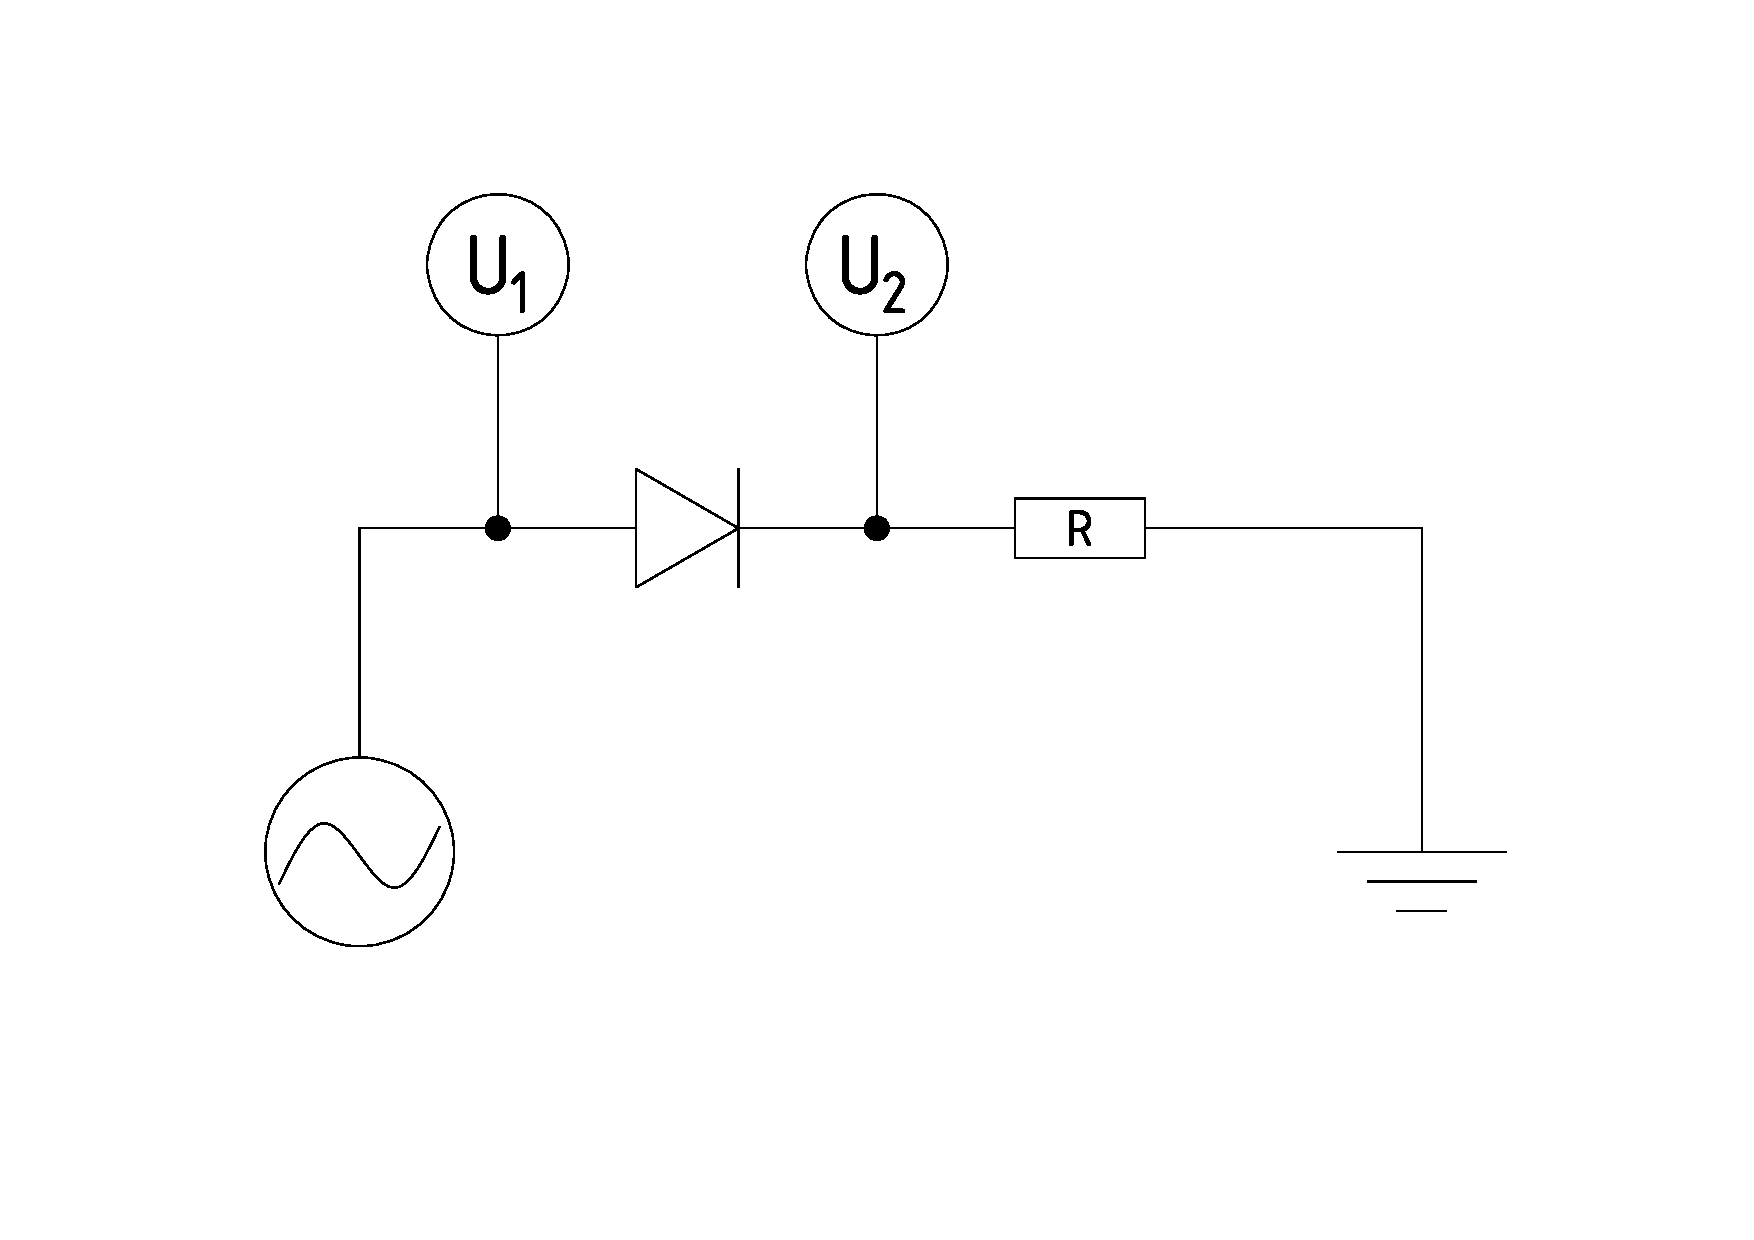
\includegraphics[width=\linewidth]{2_Experiment_Scheme}
	\caption{Электрическая схема для проведения эксперимента по получению ВАХ диодов.}
	\label{fig:2_Experiment_Scheme}
\end{figure}

\subsection{Анализ полученных результатов}

\subsubsection{Диод}

Полученные в ходе измерений данные визуализированы на рисунке \ref{fig:2_Diode}.

\begin{figure}[H]
	\centering
	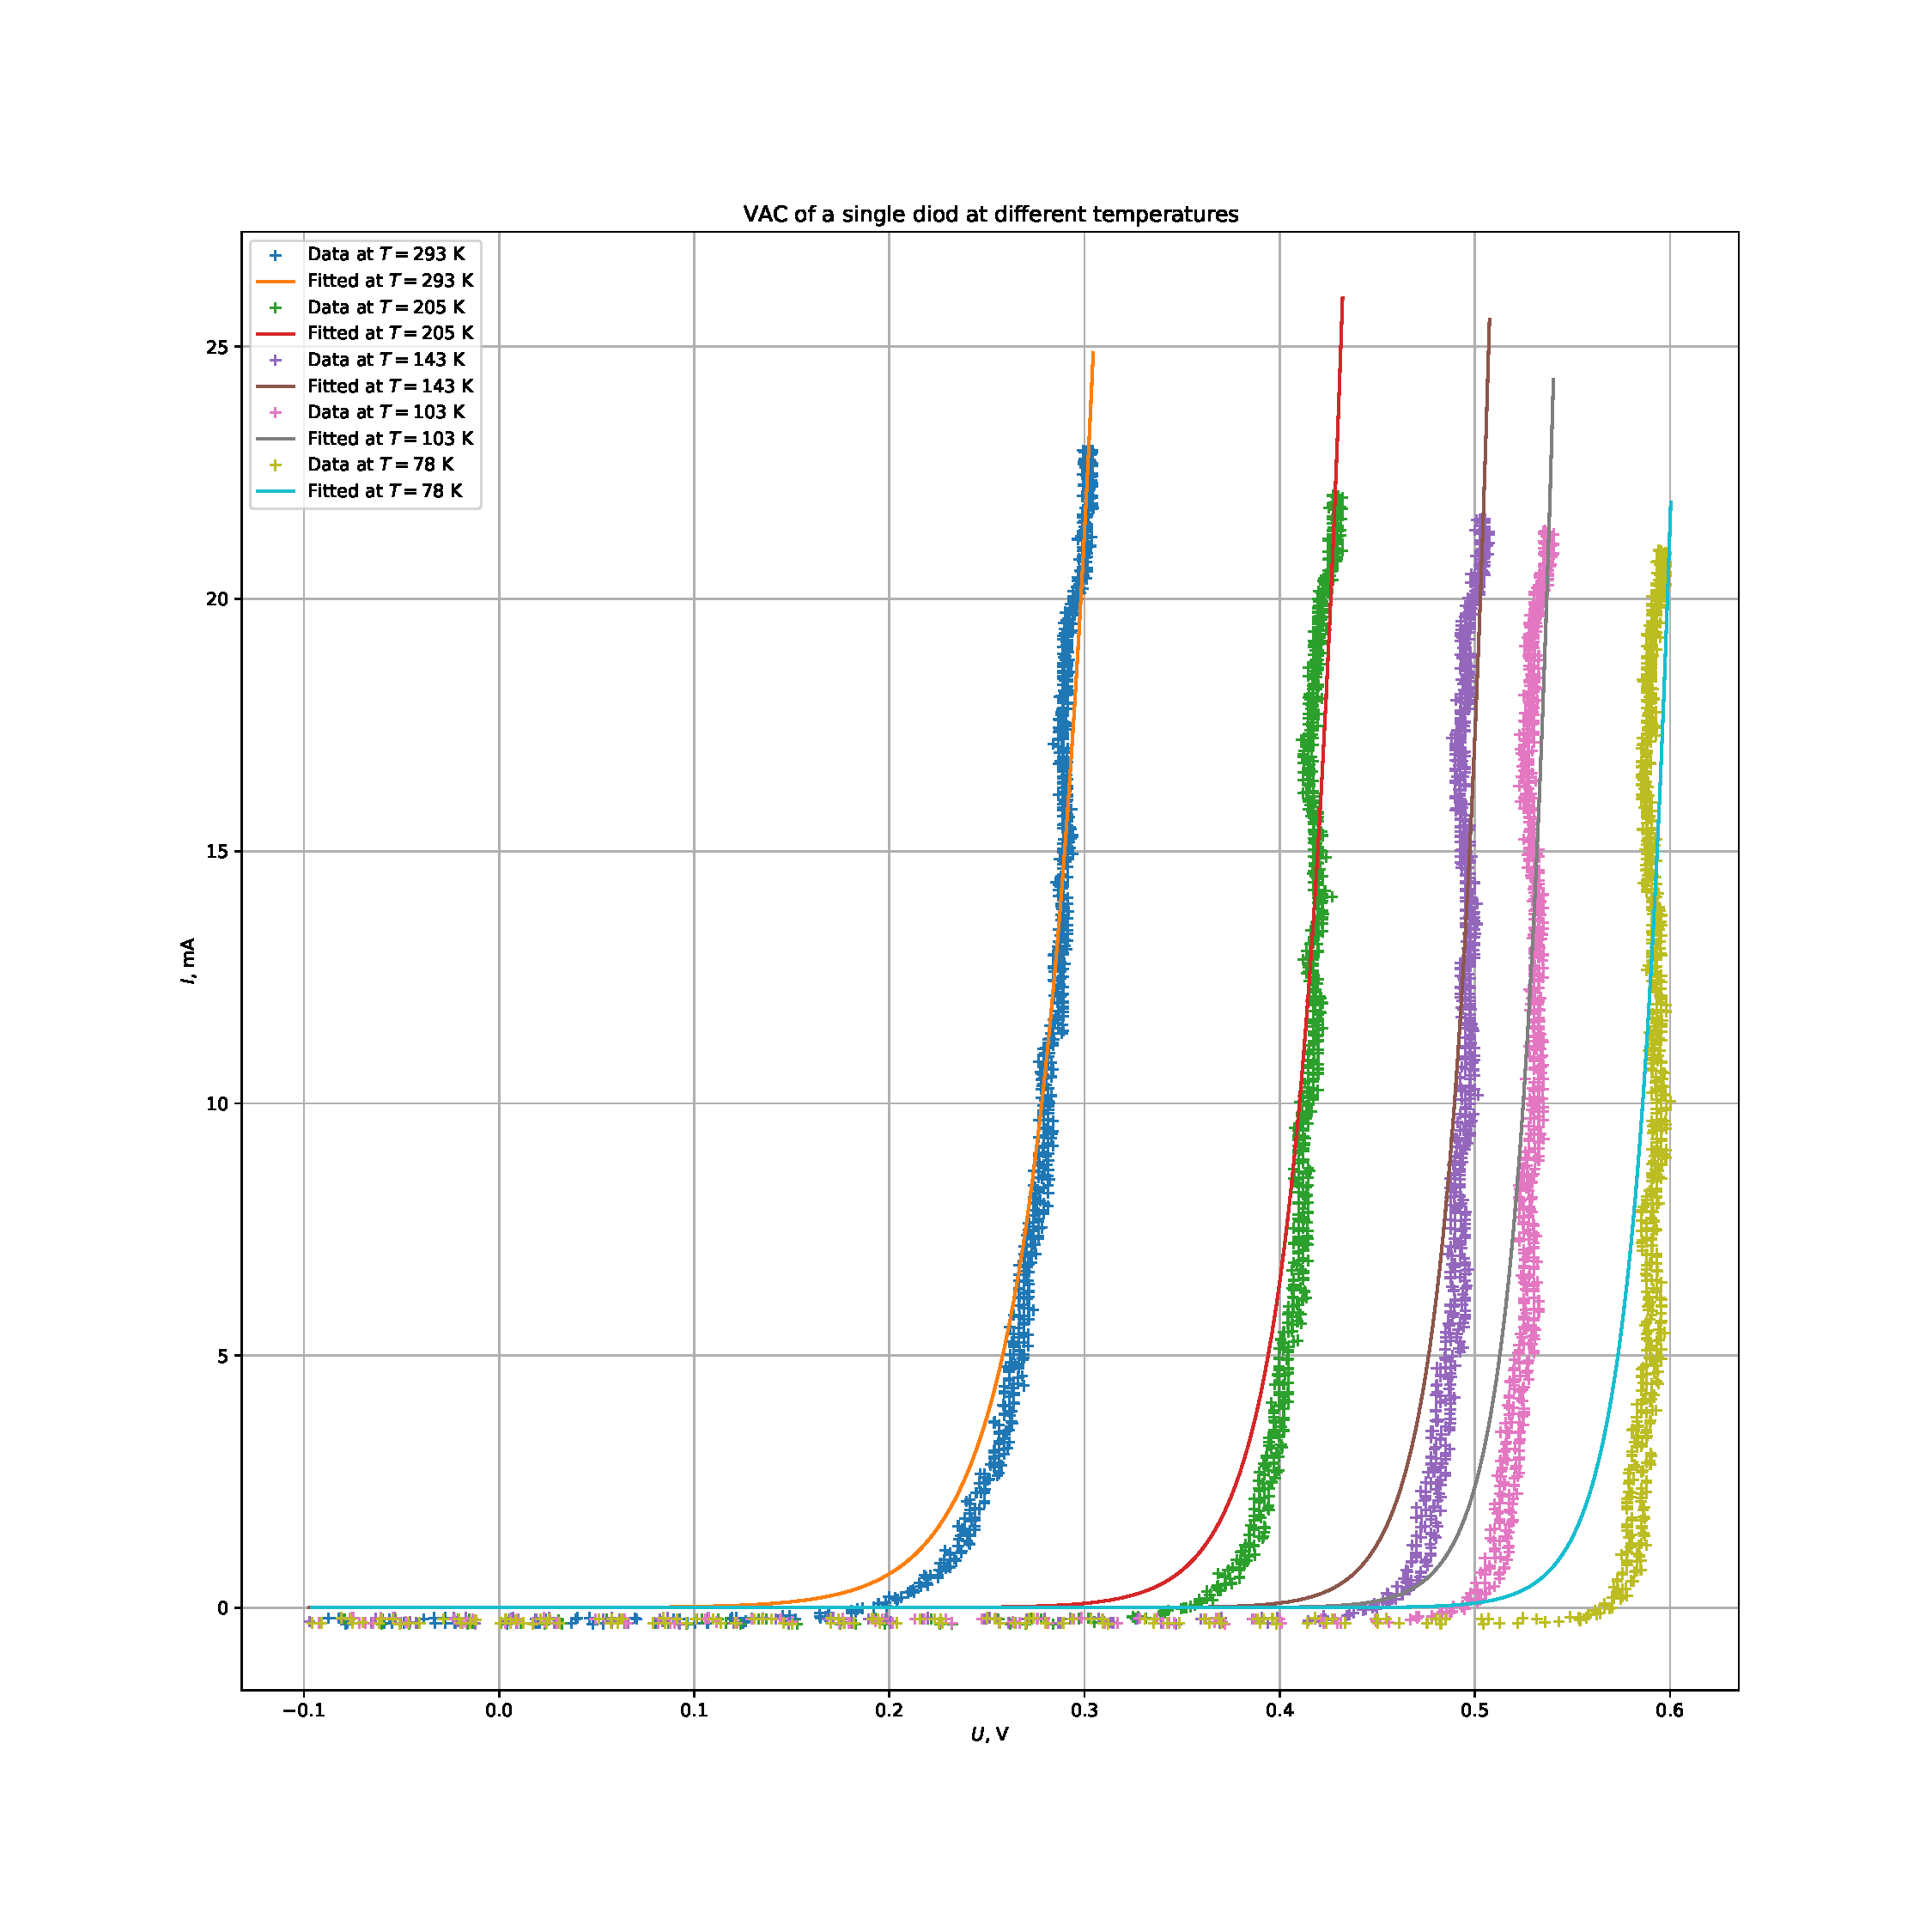
\includegraphics[width=\linewidth]{2_Diode}
	\caption{ВАХ-и диода при его различных температурах.}
	\label{fig:2_Diode}
\end{figure}

Из полученных графиков мы можем заключить, что с уменьшением температуры величина напряжения, при котором происходит открытия диода, увеличивается линейно, что видно на рисунке \ref{fig:2_Knee_Diode} и коррелирует с предсказанием теории. Кроме того, с уменьшением температуры все более резким становится скачок тока при открытии диода.

\begin{figure}[H]
	\centering
	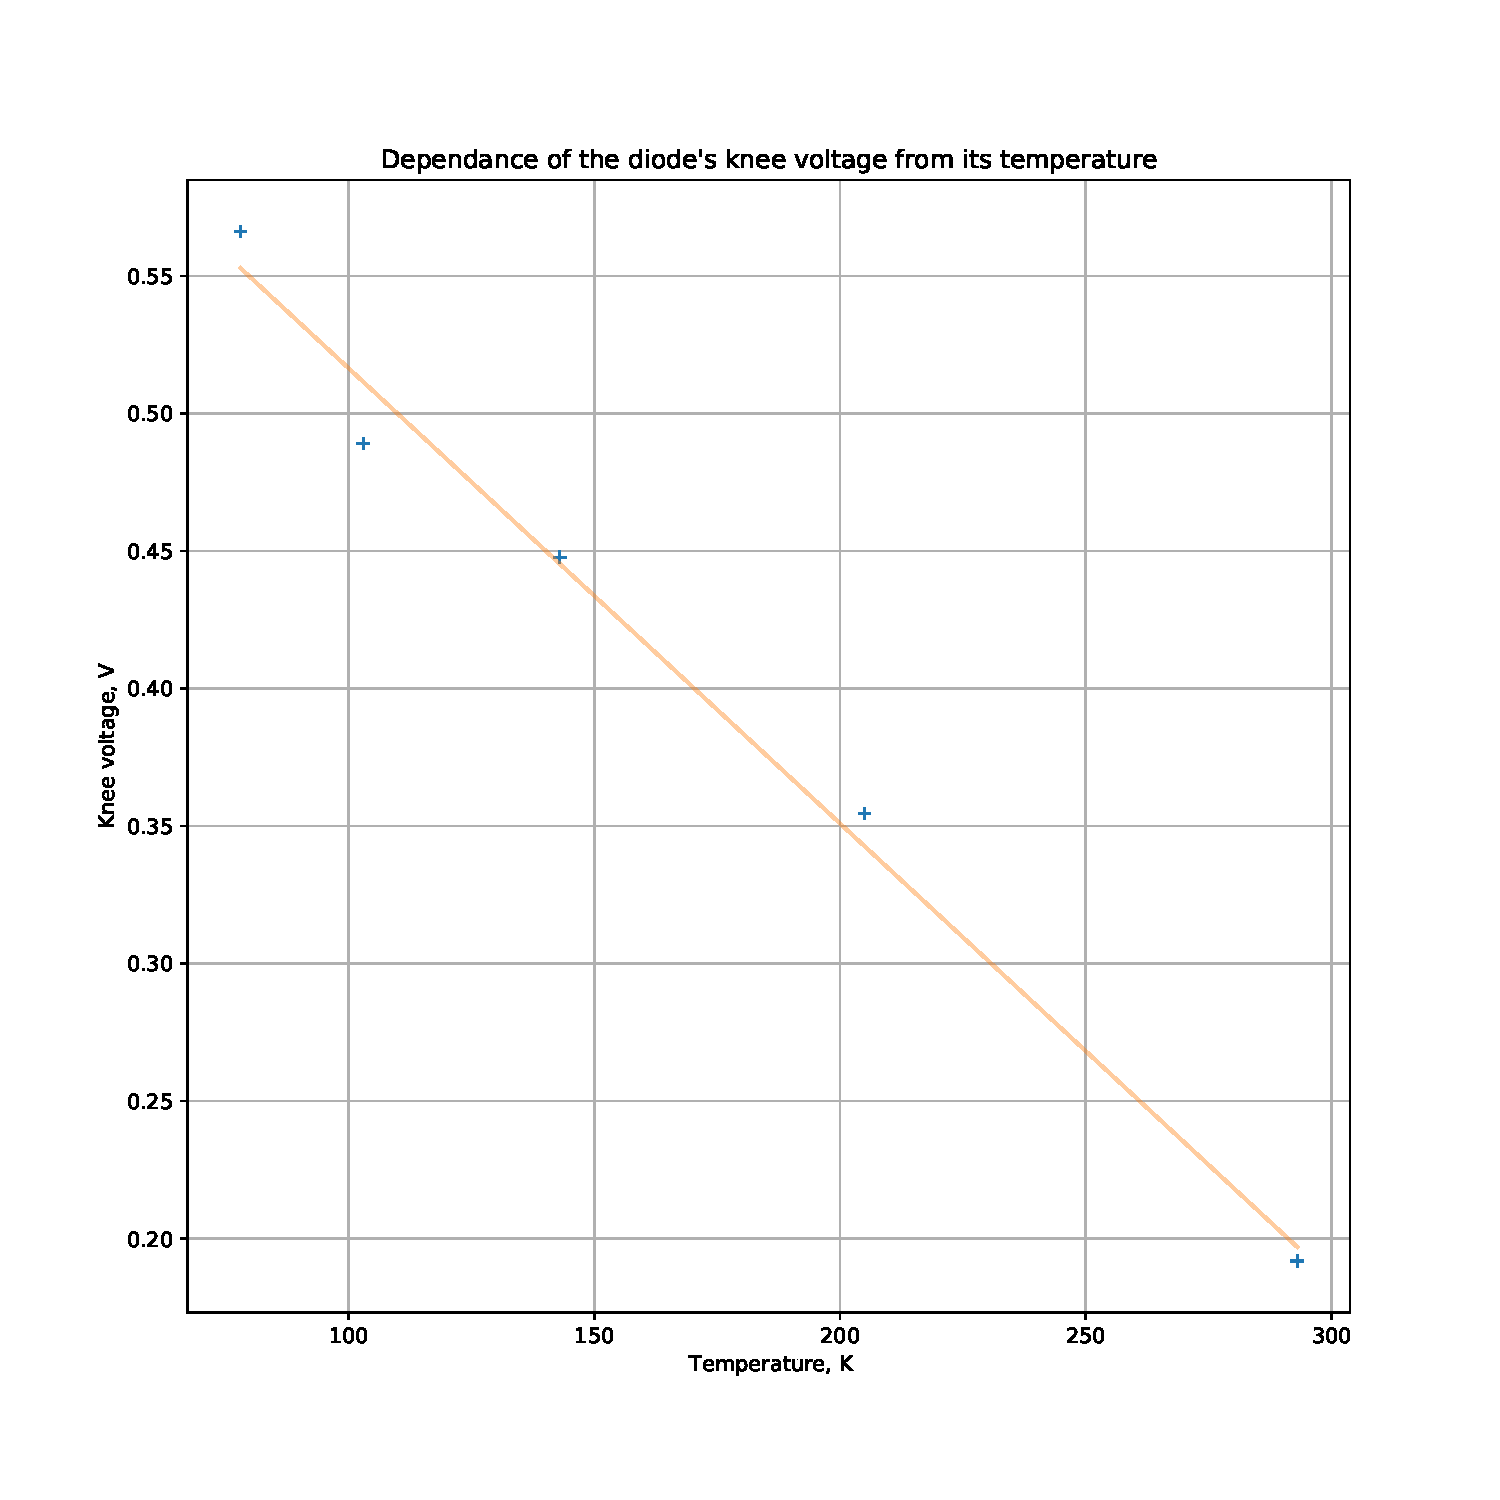
\includegraphics[width=\linewidth]{2_Knee_Diode}
	\caption{Зависимость напряжения, при котором происходит открытие диода, от его температуры.}
	\label{fig:2_Knee_Diode}
\end{figure}

\subsubsection{Светодиод}

Как и раньше, представим собранные данные на рисунке \ref{fig:2_LED}.

\begin{figure}[H]
	\centering
	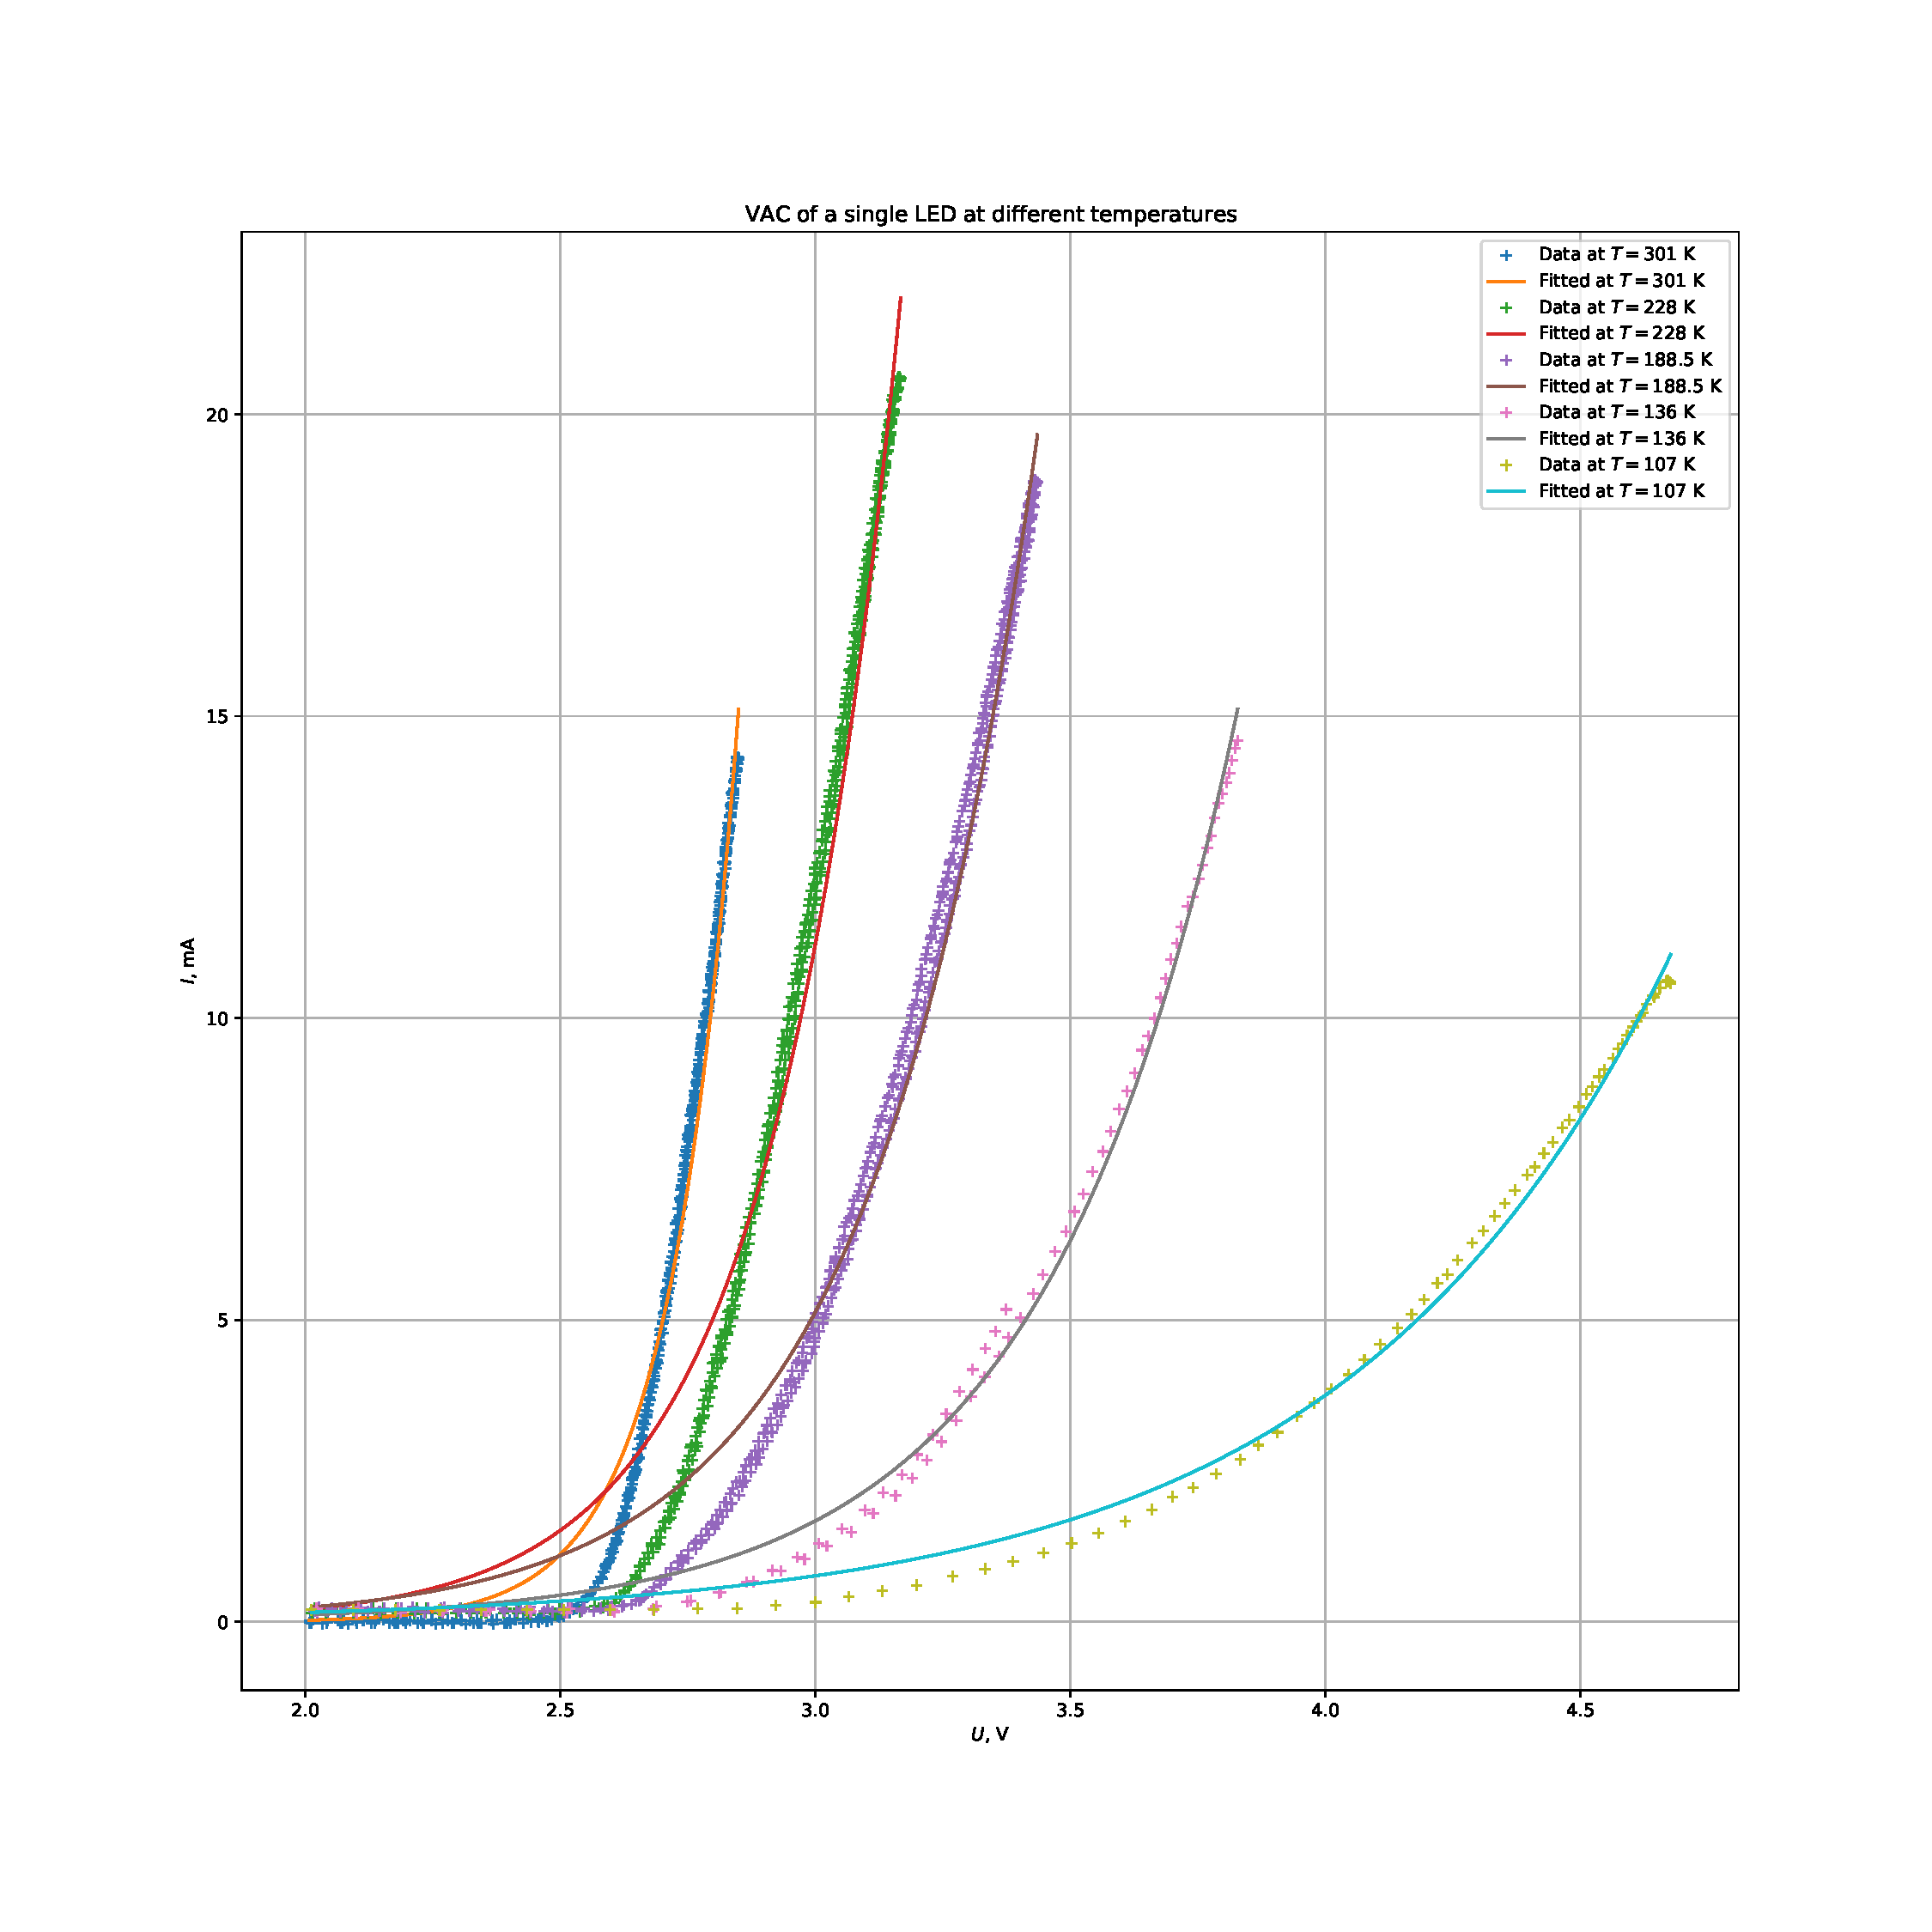
\includegraphics[width=\linewidth]{2_LED}
	\caption{ВАХ-и светодиода при его различных температурах.}
	\label{fig:2_LED}
\end{figure}

Из полученных графиков видно, что с уменьшением температуры ВАХ все больше похожа на экспоненту, в то время как ВАХ при более высоких температурах больше походят по внешнему виду на ВАХ обычного диода.


\section{Изучение эффекта Холла}




\end{document}